
\documentclass[openany]{XDBT}

\begin{document}

%%----------SURFACE----------%%

	%% Here you can fill your information:
	
	\title{西电本科毕业设计论文模板}
	%\rtitle{} %If your title is overflowed in a line, split it here. Or, ignore it. 
	\institute{计算机学院}
	\major{计算机科学与技术}
	\author{刘曜}
	\advisor{Google}
	%\class{}
	%\studentNumber{}
	\maketitle


%%----------PROLOGUE---------%%
	\frontmatter
	
\begin{abstract}

这篇文章是这个\LaTeX{}~模板的测试,我顺便写一点关于这个模板的用法。就像你现在看到的,这是一个摘要。

依据学校给的要求(已经放在附录A里了),章标题要求黑体,三号,居中;节标题要求四号,居中;其他各级标题都是小四号,黑体,居左;正文小四号,宋体,中文段落空两个字。

大概就是这些,关键字要求3-5个,中间用空格分开。

\keywords{西电~~论文~~毕业设计~~模板}
\end{abstract}

\begin{enabstract}

This is an abstract in English. I don't want to translate the content above, just a sample~~So, that's end. 

\enkeywords{Xidian~~University~~Thesis~~Template}

\end{enabstract}

	\tableofcontents

%%----------MAIN PART--------%%
	\mainmatter
	\pagestyle{content}
	\chapter{模板介绍}
\label{chap:introduction}

这个模板为2017年毕业而诞生~

因为我想用\LaTeX{}~写毕设,放寒假这几天趁小伙伴都还没回来,抽时间先写个论文模板,顺便练一下\LaTeX{}~很多用法。

这个模板我参照了一点睿思上数院一个师兄(薛继龙)的模板,但宏结构跟他写的区别不小……顺便修复了一点他的小问题,然后我的这个模板可能更custom~

\section{系统环境}
我写这个模板的系统是linux(ubuntu 16.04),文档字符集UTF-8(师兄那个是GB18030,在windows上可能不会乱码,在linux上得改配置不然会乱码)。

其次,\LaTeX{}~环境我记得我是很久以前直接装的texlive-full,然后装了个latex-cjk-chinese,好像再也没有装过其他的了,文档最终用的xelatex跑的,所以一般情况下只要装的一样,运行时不会出现少包少字体的情况。

\section{拿到模板改哪些}
首先目录结构和你需要关注的文件有这些:
\begin{itemize}
\item main.tex: 模板主文件,统筹模板的环境,和添加相应的章节,最后也是运行它。
\item partial: 这个文件夹里面*.tex的文件都是需要你自己写的(每一章写在不同文件里,可自己添加),只需要会一点点latex语法就能搞定,不需要关注版式和字体之类的,只关注内容写什么。自己添加的*.tex需要你在main.tex文件里适当的位置用$\backslash$include命令包含进去,写对路径就行。
\item graphics: 这个文件全都是图形图像文件,必须是.eps后缀,其他格式图片你可以转成.eps再放进去。有个网站很好很强大能转换,但是好像需要翻墙:\href{http://www.tlhiv.org/rast2vec/}{http://www.tlhiv.org/rast2vec/}
\item XDBT.cfg: 这里面定义了一堆常量,你可以自定义更改,但我已经按照学校要求写好了,应该不用再打开更改了。
\item XDBT.cls: 这就是宏文件,其实不用打开看,已经基本弄好了。如果想微调模板板式、字体、颜色之类的,可以在这里调,我写了比较粗糙的注释。
\item 其他文件你大部分时候都不需要关注是啥。
\end{itemize}

其次,你可能注意到了,学校也要求到,页要分左手和右手方向,奇数页左边留白多,偶数页右边留白多。有的页需要从奇数页开始(比如最后的致谢),如果它刚好是在偶数页,你可以在它之前的那一个部分的结尾加一个$\backslash$cleardoublepage用来加一个空白页。

\section{版式对齐}

现在的版式不会出现某一行太长了发生溢出的情况,因为我在XDBT.cls文件里加了几句话,主要是$\backslash$tolerance这个变量。

但现在会有一种状况,若有个特长的东西如http://www.penpineappleapplepen.com,就会让上一行的字间距特别大,就像这里的情况一样。这是无法避免的(起码我不知道)。此时就要求你能合理断句,或者在合适的地方写下比较长的部分。

师兄那个模板会出现行溢出的现象,就是写出去,像这个右侧一样
\begin{figure}[h]
 \centering
	\fbox{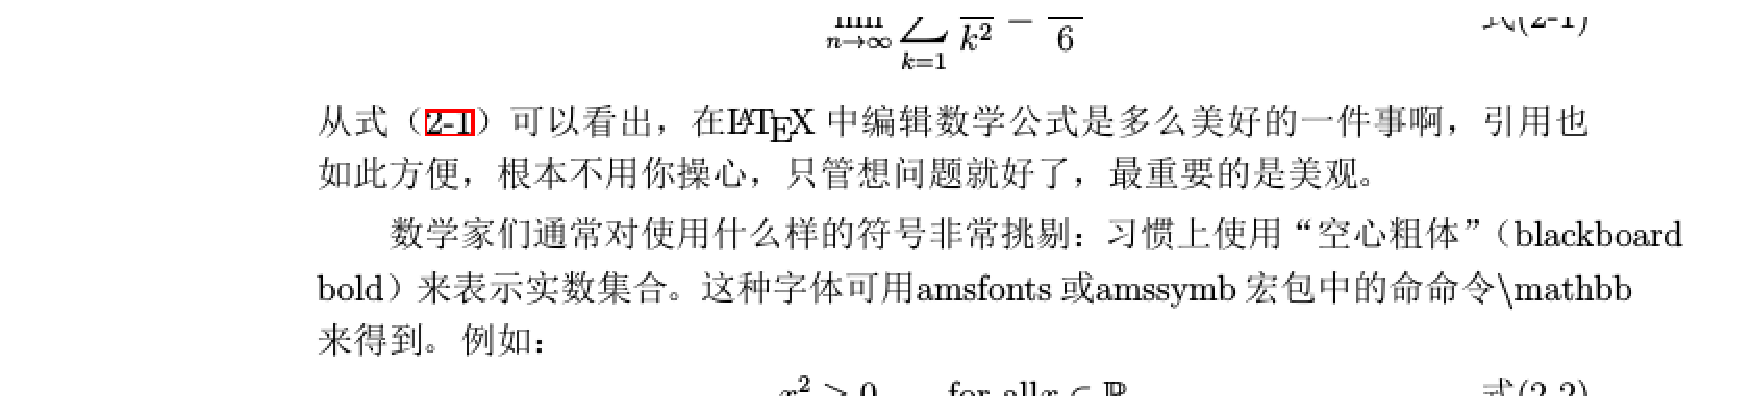
\includegraphics[width=1\textwidth]{overflow}}
 \caption{行溢出}
 \label{fig:amss1}
\end{figure}

这样的话,也是需要你在适当的地方换行。如果你想用他这种,自己写的时候稍微注意一下也可以,你只需要把上面那个变量注释掉就行了。

\section{版权问题}

尊重版权,保证自由,鼓励开源,不建议收费- -

GNU License

\section{问题反馈}

如果模板有问题,你可以自己改改,我也欢迎和我讨论交流:

\href{derektanko@gmail.com}{derektanko@gmail.com}

祝各位顺利毕业,升职加官,当CEO,娶白富美(or嫁高富帅),早得贵子,延续人类,(入土为安)。
	
\chapter{数学相关}
\label{chap:math}
我稍微写写关于数学相关的语法,测试一下模板是否运行正确。
\cite{mycite}。

\section{公式}

\begin{itemize}
    \item 行内的公式一般用\$和\$,这两个之间夹着你要写的内容,示例:这样的写法(顺便也把代码块的写法测试了- -,代码块的样式在XDBT.cls里面有定义)%
    \begin{lstlisting}
    $a^2+b^2=c^2$
    \end{lstlisting}
    会得到$a^2+b^2=c^2$
    \item 行间公式用\$\$和\$\$,示例:
    \begin{lstlisting}
    $$a^2+b^2=c^2$$
    \end{lstlisting}
    会得到$$a^2+b^2=c^2$$
    \item 还有带编号的公式,我就不写代码了,你可以去看这个模板源码,效果:
    \begin{equation}\label{eq:lim}
        a^2+b^2=c^2
    \end{equation}
\end{itemize}

\section{定理和定义}
同样不贴代码了,只有演示效果
\begin{thm}
我是一个小定理~
\end{thm}

\begin{thm}
我是另一个小定理,带公式的小定理~
\begin{equation}
    a^2+b^2=c^2
\end{equation}
\end{thm}

\begin{algo}
我是一个小算法~
\end{algo}






	
\chapter{表格图形}
\label{chap:tabfig}

\section{表格}
示例1,中间有竖线的:
\begin{center}
\begin{tabular}[t]{l|c}
    \hline
    姓名 & 战斗力 \\
    \hline
    习XX & 999 \\
    蛤XX & 9999 \\
    川普 & 0.1 \\
    \hline
\end{tabular}
\end{center}


示例2,中间没竖线的:
\begin{table}[htbp]
 \caption{\label{tab:test}示例表格}
 \centering
 \begin{tabular}{lcl}
  \toprule
    姓名 & 战斗力 \\
  \midrule
    习XX & 999 \\
    蛤XX & 9999 \\
    川普 & 0.1 \\
  \bottomrule
 \end{tabular}
\end{table}

\section{图形}
这玩意儿好像只能加eps的图,前面提到了,也给转换工具的网址了

示例:
\begin{figure}[h]
 \centering
 \includegraphics[width=0.3\textwidth]{xdSign}
 \caption{这是一个图片}
 \label{fig:amss1}
\end{figure}




	\appendix
\titleformat{\chapter}[hang]{\heiti\bfseries\center\zihao{3}}{附录{\thechapter}}{1em}{\zihao{3}}
	\include{partial/A-rules}

%%----------ACCESSORY--------%%
    \backmatter
    
\begin{thanks}

这就是一个致谢页面,通常你要在这里把你身边认识的人都问候一遍。举个例子:

谢谢祖国,谢谢陕西,谢谢长安,谢谢爸爸,谢谢妈妈,谢谢西电校园,谢谢西电所有老师,谢谢西电所有同学,谢谢楼管,谢谢综合楼,谢谢西电流浪狗,谢谢西电流浪猫,谢谢西电其他流浪的动物,谢谢lol,谢谢DotA,谢谢炉石,谢谢其他游戏,谢谢麒麟臂,谢谢大家,让我在西电这个校园活着度过了这四年,god bless you,今当远离,临表涕零,不知谓何,特此鸣谢。

哦,论文啊,已经写完了,我能毕业了吧?谢谢谢谢审核老师,祝你鸡年大吉!

......

\vskip 18pt

2017-01-17

\end{thanks}

\cleardoublepage

    
\fontsize{10.5pt}{10.5pt}\selectfont
\begin{thebibliography}{10}

\bibitem{mycite}
这是一个引用的示例
\newblock {附件里有个关于数学语法的详细讲解.pdf}.
\newblock (2017)


\end{thebibliography}


\end{document}